\subsection{Habilitations}
\vspace{1cm}

Un autre critère essentiel à la mise en place de l’automatisation de la désignation des arbitres était la prise en compte des habilitations des arbitres. En effet, cet algorithme devait pouvoir proposer la désignation d’arbitres habilités pour chaque match.

Le problème était que ces habilitations n’étaient pas disponibles directement dans les informations liées aux arbitres, et ne pouvaient pas être récupérées via CURL comme pour les informations précédentes. Il fallait donc pouvoir récupérer celles-ci d’une façon différente.\\

Ici encore j’ai pensé à deux méthode qui présentaient chacune leurs avantages et inconvénients :

\begin{itemize}
    \item la première méthode était de déduire ces habilitations à partir de la liste passée des désignations, en prenant en compte le type de match le plus élevé qu’avait arbitré chaque arbitre, pour en déduire un plafond d’habilitation.
    \item La deuxième méthode était de déduire les habilitations de chaque arbitre à partir du grade et du niveau de leur licence.
\end{itemize}

La première méthode présentait quelques problèmes : le plus important était le manque d’informations concernant une bonne partie des arbitres qui n’avaient pas pu arbitrer les matchs de la saison en cours. De plus, les arbitres pour lesquels les informations étaient disponibles ne reflétaient pas forcément le niveau maximum d’habilitation qu’ils possédaient. J’ai estimé un taux d’erreur avec cette méthode de l’ordre de 30\% environ.\\

Concernant la deuxième méthode, il faut savoir que les habilitations d’arbitres ne sont pas toujours définies par leur niveau et grade de licence, mais que ces données sont quand même fortement liées aux habilitations. Le taux d’erreur avec cette méthode était de l’ordre de 15\%.\\

Le taux d’erreur étant plus faible, j’ai donc décidé de me reposer sur la deuxième méthode pour effectuer la déduction des habilitations, et de mettre en place une interface graphique permettant la mise à jour de celles-ci.  Cette interface permettrait aux gestionnaires d’effectuer les modifications nécessaires pour les arbitres pour lesquels les habilitations ne correspondraient pas.

Pour effectuer la mise en place des habilitations initiales des arbitres, j’ai créé une unique méthode dans une classe dédiée à cette tâche

\newpage

\begin{figure}[!h]
    \centering
    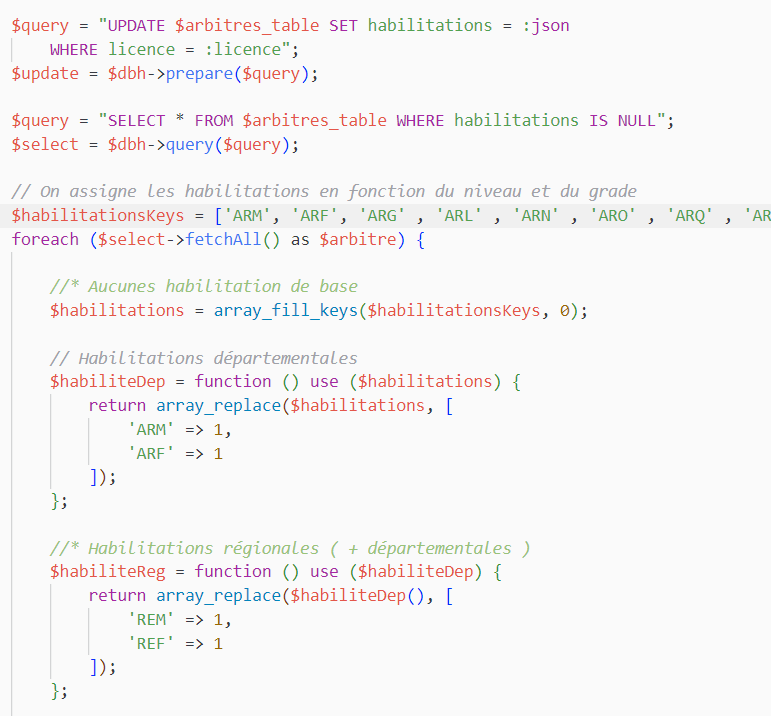
\includegraphics[width=10cm]{habilitations_code.png}
    \caption{Mise en place des requêtes et fonction nécessaire à la mise en place des habilitations}
\end{figure}

\begin{figure}[!h]
    \centering
    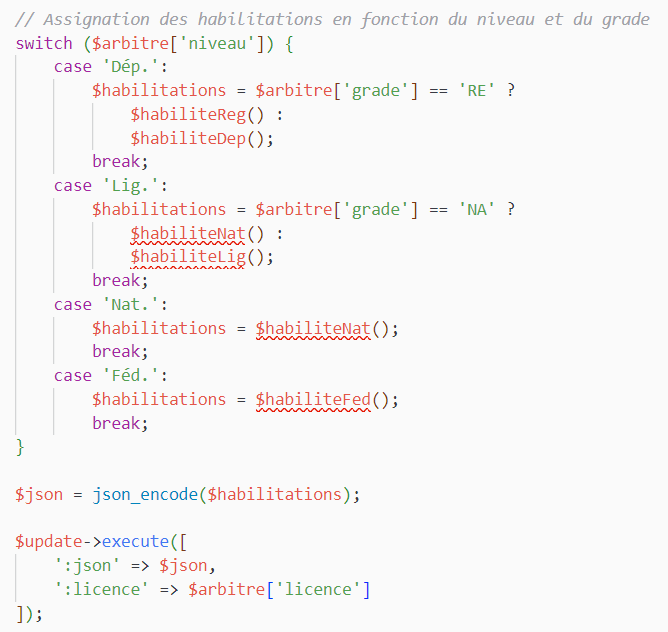
\includegraphics[width=10cm]{habilitations_code2.png}
    \caption{Détermination des habilitations initiales de l'arbitre}
\end{figure}

\newpage 

Les différents types d’habilitations nous ont été indiqués par notre tuteur et sont définis par des critères subjectifs basés sur les différents types de matchs possibles. Les clés correspondantes à ces habilitations sont stockées dans un tableau indexé, et initialisées à zéro pour chaque arbitre. Cette valeur signifie que les arbitres n’ont aucunes habilitations au départ.  

Puis en fonction du niveau et du grade de leur licence, les habilitations des arbitres sont modifiées à un pour chaque clé correspondante au niveau d’habilitation associé. Ces habilitations étant cumulées de façon croissante à chaque niveau supplémentaire, j’ai utilisé la fonction \colored{array\_replace()} pour retourner un tableau des habilitations complètes de chaque arbitre.

Une fois ce tableau défini, il fallait finalement l’insérer sous format \colored{JSON} dans la base de données. Pour faire cela, j’ai utilisé la méthode \colored{json\_encode()} sur le tableau des habilitations et je l’ai inséré à l’aide d’une requête SQL de type INSERT. \\ \\ 

Une fois les habilitations initiales insérées dans la base de données, j’ai ensuite pu travailler sur l’interface de mise à jour de celles-ci. 
J’ai donc mis en place une page annexe qui affiche la liste de tous les arbitres, auxquels on associe la liste de toutes les habilitations préremplies sous forme de SELECT. Chaque select permet de choisir entre “Oui/Non”, permettant ainsi de choisir ou non d’accorder l’habilitation à l’arbitre voulu. 

\begin{figure}[!h]
    \centering
    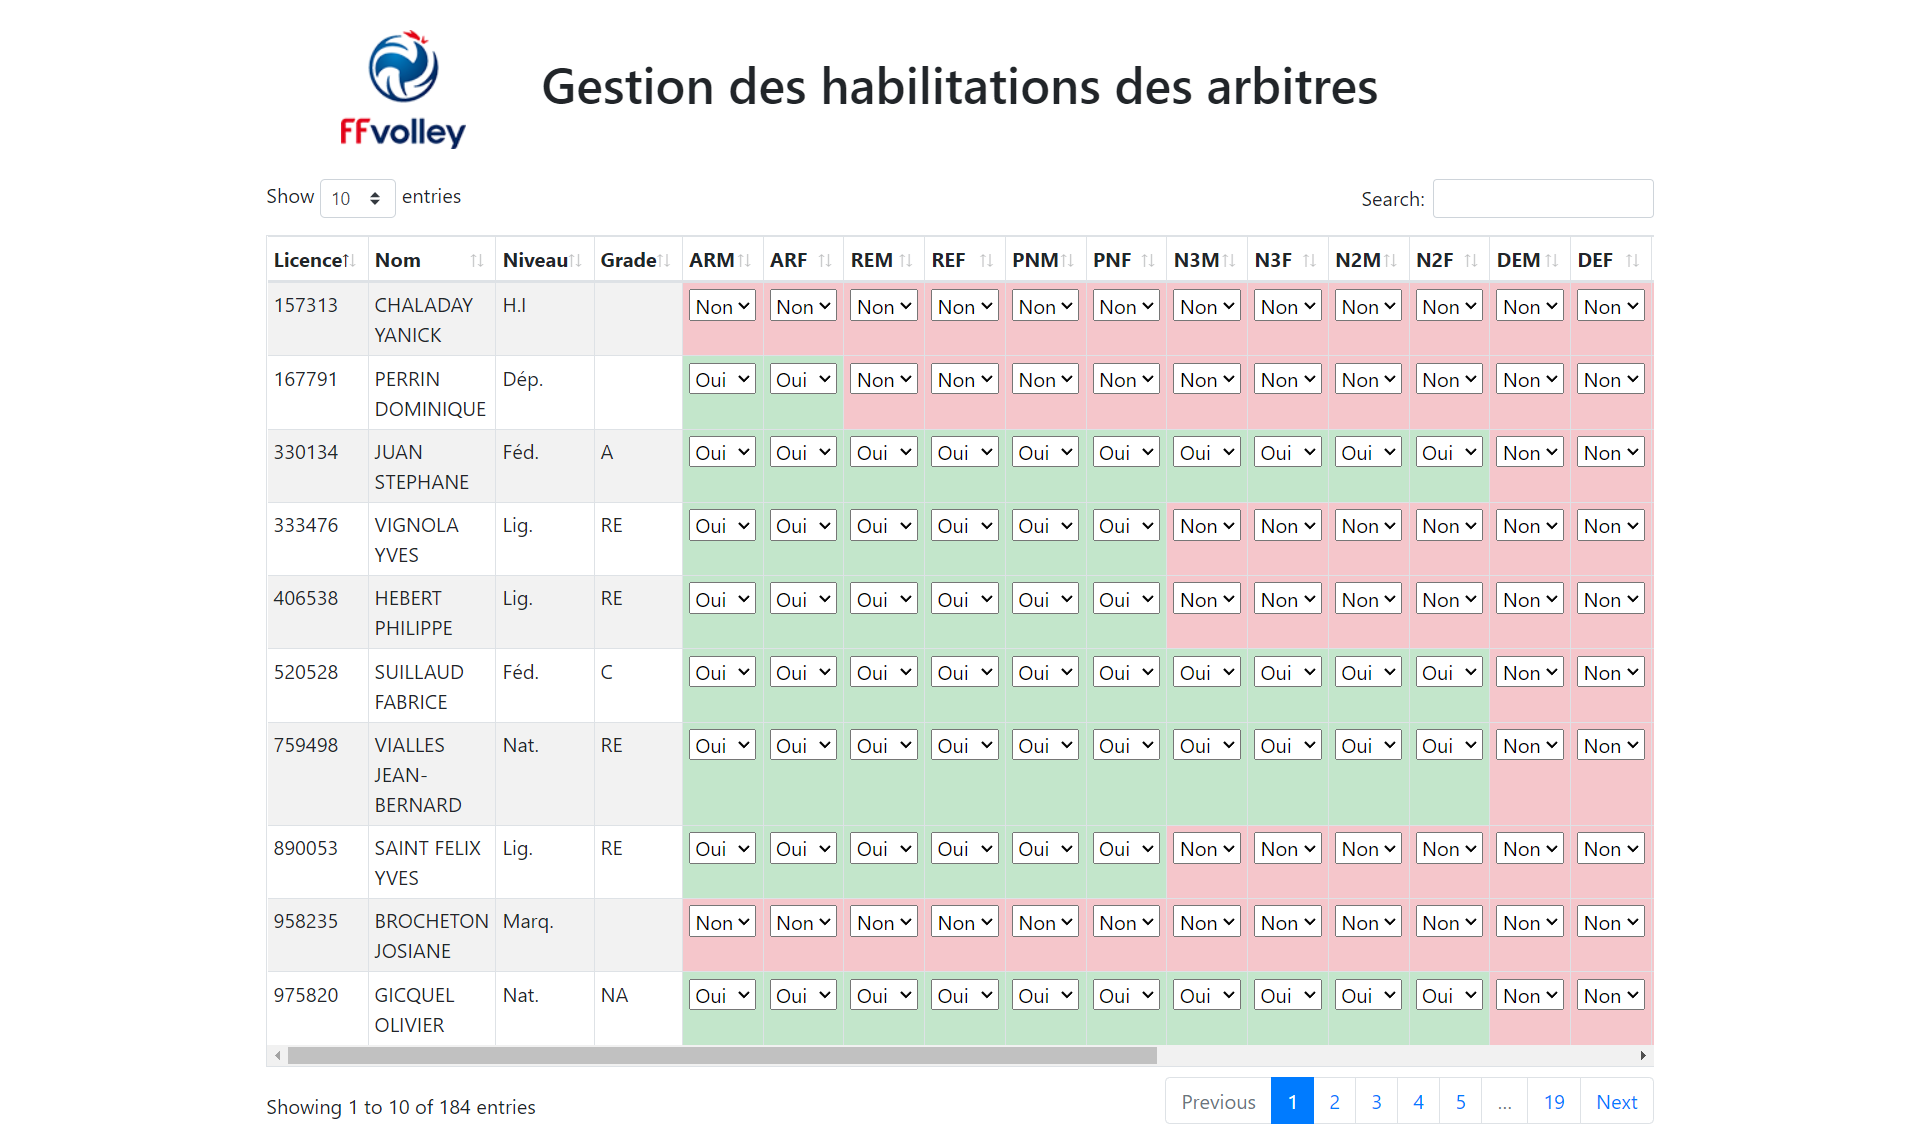
\includegraphics[width=\linewidth]{habilitations.png}
    \caption{Interface de mise à jour des habilitations}
\end{figure}

\newpage

Un script javascript permet ensuite au changement d’un select, d’envoyer via ajax le numéro de licence et les nouvelles informations d’habilitations à une page dédiée de notre back-end. Cette page récupère ensuite les habilitations actuelles de l’arbitre, les transforme en tableau associatif grâce à la fonction \colored{json\_decode()}, puis met à jour l’habilitation voulue. Elle encode ensuite ce nouveau tableau sous format JSON et l’insère dans la base de données.

Pour plus de détails concernant la partie graphique de cette page, merci de vous reporter au chapitre sur les interfaces.